\chapter{设计思路及实现过程}
\section{程序整体框架}
整个程序利用了acllib库的API来完成,acllib其底层还是用到windows.inc的许多东西,但使用起来更加顺手简洁。
\par
程序的运行结构和利用windows.inc的那种消息派发解释循环的结构类似,也有其固定格式:在init\_first,init\_second间画好主界面,先设置初始化窗口initWindow:
\begin{lstlisting}[language={[x86masm]Assembler}]
    main proc c
        invoke init_first  ;初始化绘图环境
        invoke initWindow, offset winTitle, 250, 30, 800, 600 ;左上角的坐标,窗体的宽高
        ...
        invoke start_menu;画初始菜单以及初始值
        invoke init_second
    main ENDP
    END main
\end{lstlisting}
\par
注册三个类,分别有键盘、鼠标、和计时器类用于触发事件(在之后具体解释)。
\par
画游戏的主菜单页面是在子程序里。
\par
计时器类依据不同的标志变量,来调用不同的函数,程序调用draw\_game不断更新。
\par
鼠标类用来触发点击事件:在鼠标点击后获得点击坐标,判断位置如果在start处则开始游戏,调用游戏的初始化设置,以及调用触发计时器,以30ms为间隔来不断触发更新。
\par
人物结构,子弹结构,道具结构的初始化,有关位置、大小、方向、速度的问题。而对于道具的初始化,则要用到一个随机函数来完成:
\begin{lstlisting}[language={[x86masm]Assembler}]
    getRand proc c uses ecx edx rand_num: dword
        ;设置随机种子
        push 0
        call crt_time
        add esp,4

        add eax,seed
        mov seed,eax;seed更新
        
        push eax
        call crt_srand
        add esp,4

        invoke crt_rand
        mov edx, 0
        mov ecx, rand_num
        div ecx
        mov eax, edx;返回余数
        ret
    getRand endp
\end{lstlisting}
\par
getRand中的原理是:利用时间做种子,来生成随机数。但由于汇编中执行速度非常快,在最初的时候,由于时间种子一样,得到的位置是一致的。最后解决方法为不用时间做种子,自己定义了一个seed,在每次调用getRand时做更新,因此得到了每次不同的值。
\par
键盘类用来触发人物的有子弹时发弹、无子弹时改变方向的事件。
\section{设计思路和实现过程}
在设计的过程中,我们对程序的功能进行了分解。主要将其按照页面和逻辑划分。分为主菜单页面、正式游戏页面、游戏结束页面。在主菜单页面中,主要需要实现页面跳转逻辑、图片插入逻辑,需要维护一个按钮结构体;在正式游戏页面里,主要需要实现图片插入逻辑、图片切换逻辑、人物和子弹移动逻辑、道具功能逻辑、子弹射中判定逻辑、事件响应逻辑,需要维护人物属性结构体、子弹属性结构体、道具属性结构体。主菜单页面和正式游戏页面的衔接过程由页面跳转逻辑实现。正式游戏页面和游戏结束页面的跳转过程由子弹射中判定逻辑后对游戏人物生命值的调整来实现。
\begin{figure}[htbp]
    \vspace{13pt} % 调整图片与上文的垂直距离
    \centering
    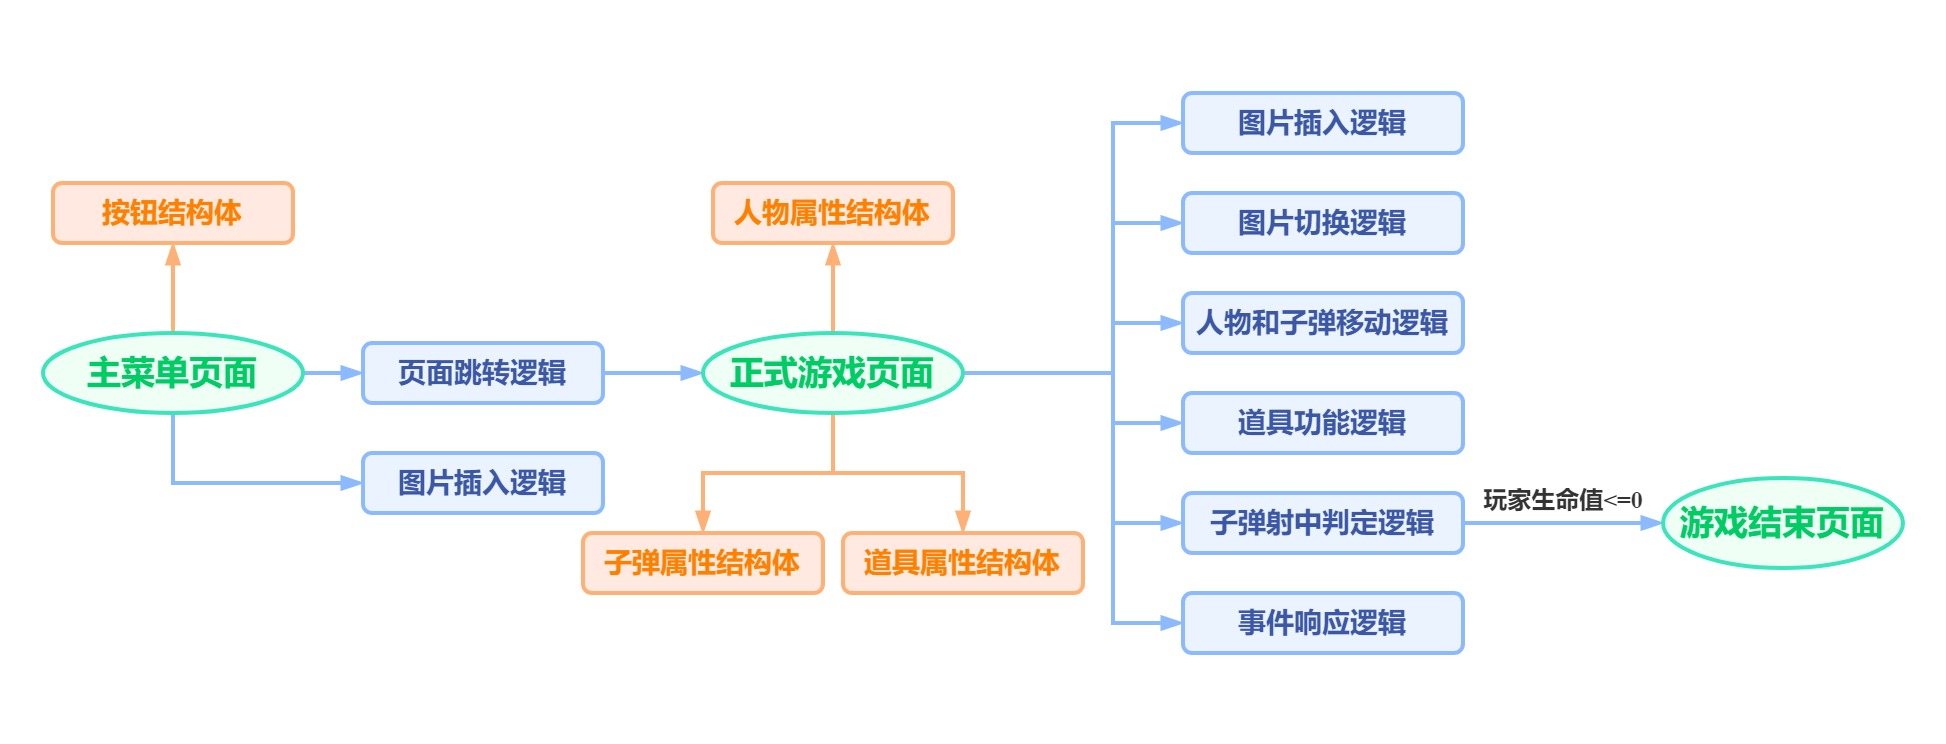
\includegraphics[width=0.8\textwidth]{images/3-1.jpg}
    \caption{游戏逻辑设计分解图}% label 用来在文中索引
\end{figure}
\subsection{页面跳转逻辑}
页面跳转逻辑主要控制游戏中的各种界面的衔接。游戏主要有两个页面,第一个是主菜单页面,第二个是正式游戏页面。主菜单页面作为打开游戏后,玩家能看到的第一个界面,拥有的最主要的功能就是作为一个首界面,实现向正式游戏页面跳转的逻辑。在主菜单页面中,设置两个按钮,一个为“Start”,一个为“Exit”。“Start”按钮在点击后的功能是跳转去“正式游戏页面”。“Exit”按钮在点击后的功能是退出程序运行。
\begin{figure}[htbp]
    \vspace{13pt} % 调整图片与上文的垂直距离
    \
    \centering
    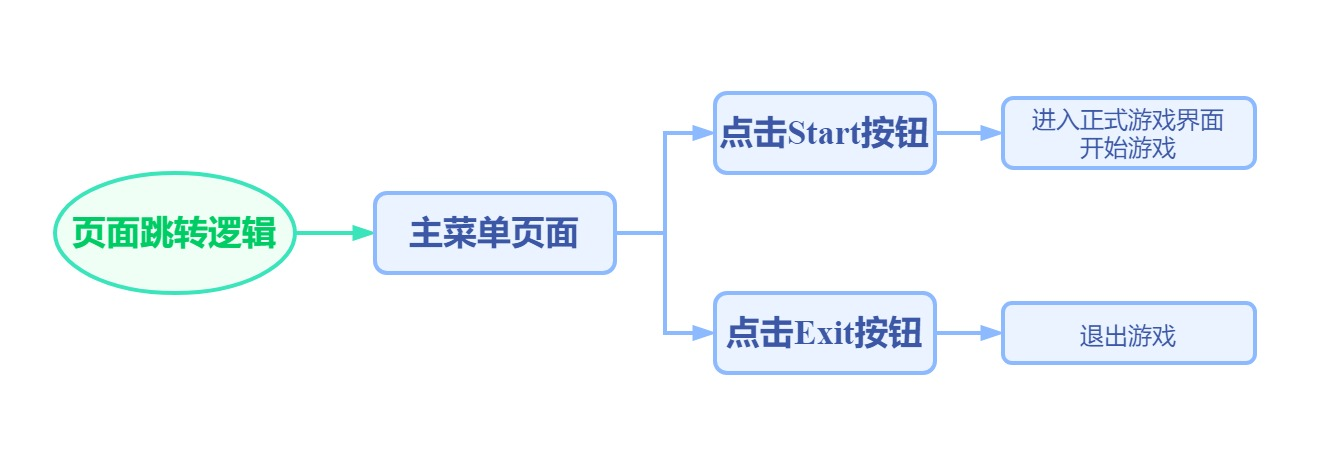
\includegraphics[width=0.8\textwidth]{images/3-2.jpg}
    \caption{页面跳转逻辑示意图}% label 用来在文中索引
\end{figure}
\par
当前界面需要维护的是一个结构体类型MyButton,它的任务是记录当前结构体变量的图片范围——左边界left、右边界right、上边界top、下边界bottom。在具体的代码实现中,定义为start\_button和exit\_button两个结构体变量。
\begin{lstlisting}[language={[x86masm]Assembler}]
    MyButton struct
        top	dd	?
        left	dd	?
        right	dd	?
        bottom	dd	?
    MyButton ends
\end{lstlisting}
\par
页面跳转部分主要依靠全局变量curWindow来控制。在当前页面为主菜单页面时,为curWindow赋值为0;如果当前页面为正式游戏页面,则为curWindow赋值为1。
\subsection{图片插入逻辑和图片切换逻辑}
图片插入逻辑主要控制的是游戏中的界面美观程度和游戏的视觉体验感。在对图片进行制作和处理后,我们确定了所有要插入图片的位置和图片素材,绘制了每个页面的各个图片素材应该出现在的位置的示意草图。
\begin{figure}[htbp]
    \vspace{13pt} % 调整图片与上文的垂直距离
    \centering
    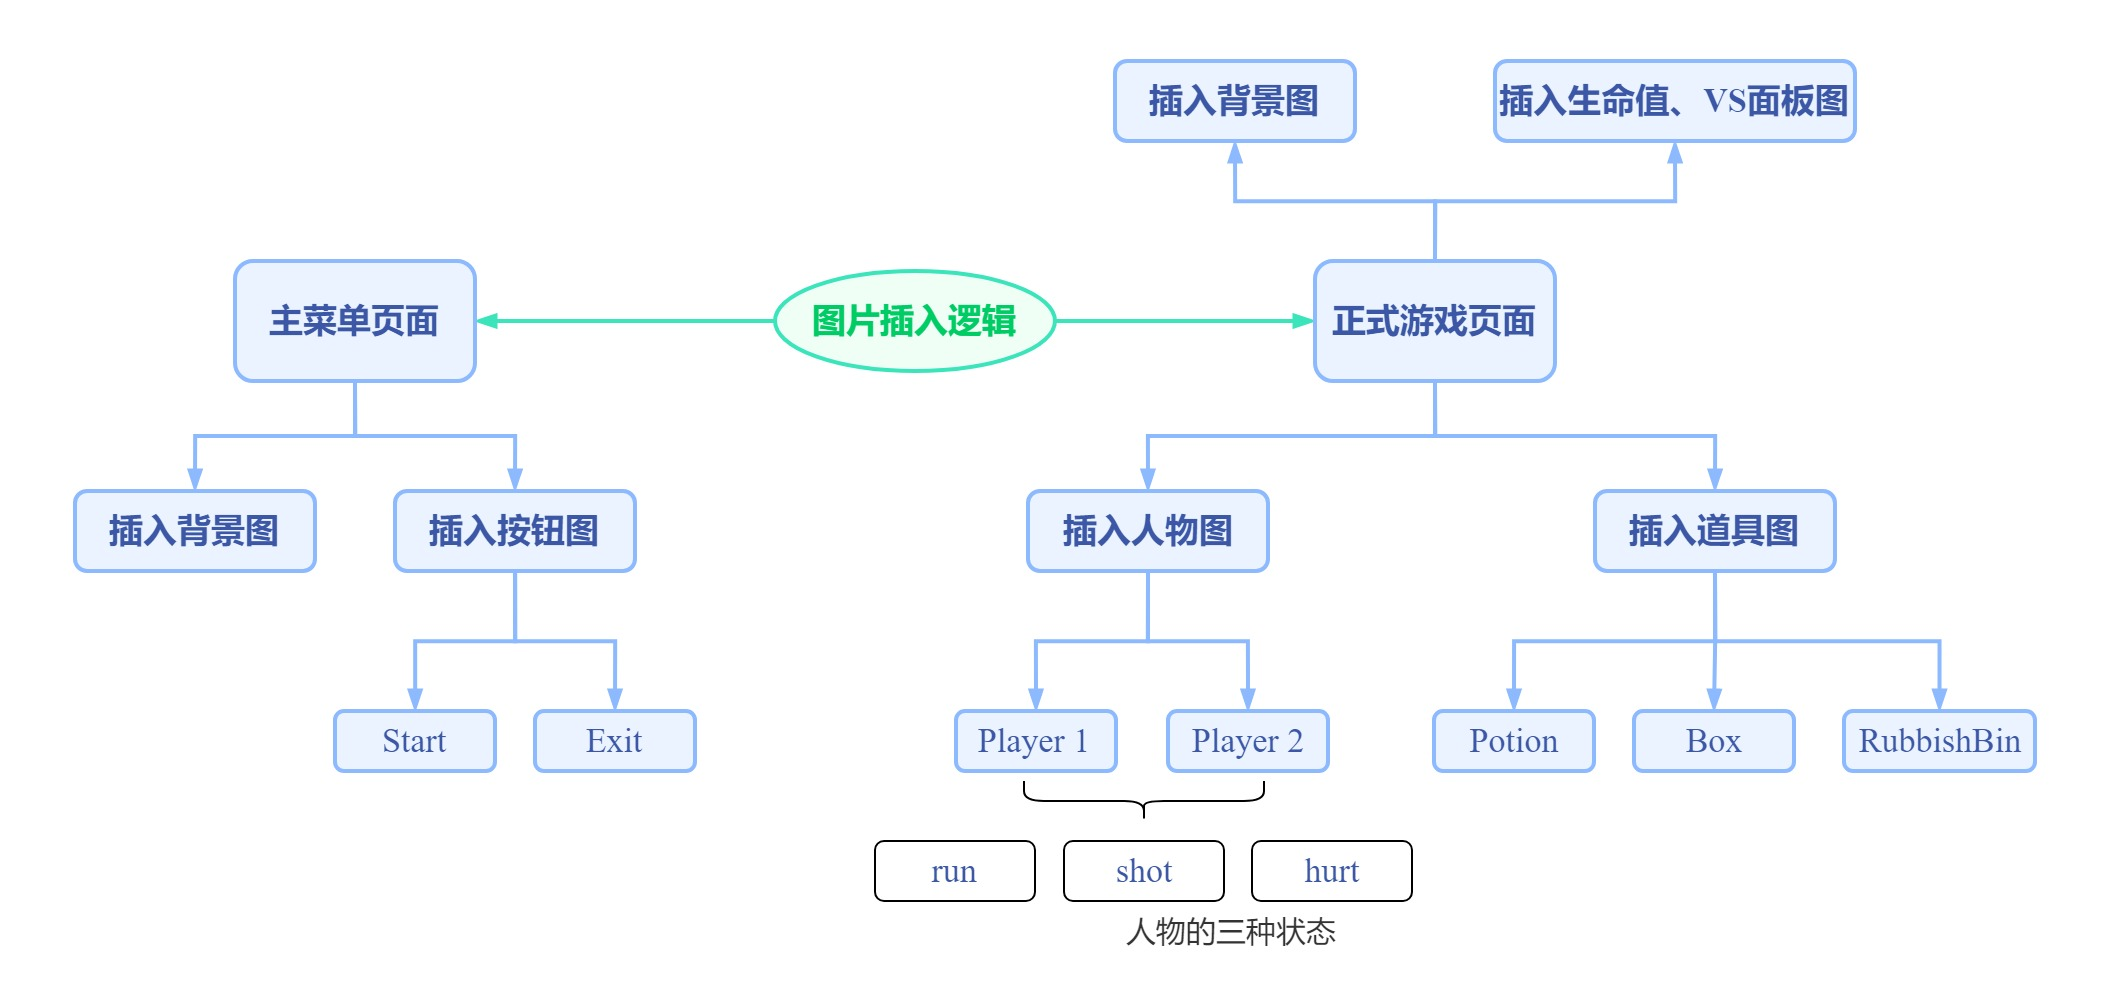
\includegraphics[width=0.7\textwidth]{images/3-3.jpg}
    \caption{图片插入逻辑示意图}% label 用来在文中索引
\end{figure}
\begin{figure}[htbp]
    \vspace{13pt} % 调整图片与上文的垂直距离
    \centering
    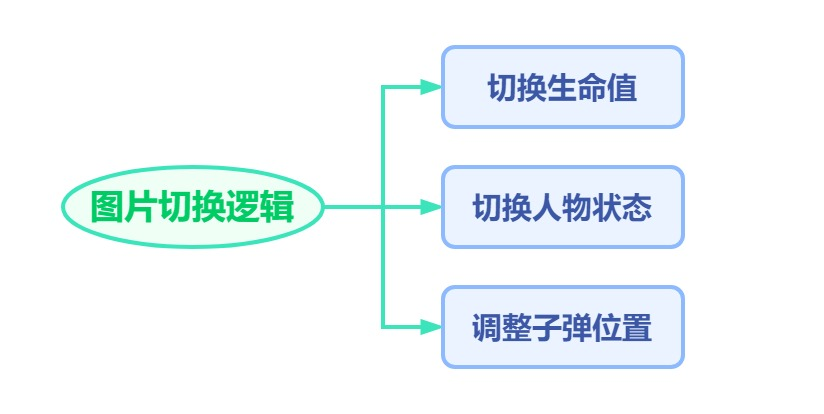
\includegraphics[width=0.5\textwidth]{images/3-4.jpg}
    \caption{图片切换逻辑示意图}% label 用来在文中索引
\end{figure}
\par
我们把图片分为五类,分为按钮、背景、子弹、人物、道具。
\par
主菜单页面只关注主菜单背景图和“Start”、“Exit”按钮图的绘制,因此在start\_menu子程序中,对主菜单页面进行绘制即可,并且在这里加入判断标识curWindow=0,用来表示这是主菜单页面。
\begin{lstlisting}[language={[x86masm]Assembler}]
    start_menu proc C
        ;载入图片
        invoke loadImage, offset page1_Bg, offset imgBg
        invoke loadImage, offset page1_Title, offset imgTitle
        invoke loadImage, offset page1_Start, offset imgStart
        invoke loadImage, offset page1_Exit, offset imgExit	

        ;显示主界面
        invoke beginPaint
        invoke putImageScale, offset imgBg, 0, 0, 800, 600
        invoke putImageScale, offset imgTitle, 200, 100, 400, 100
        invoke putImageScale, offset imgStart, 260, 300, 240, 100
        invoke putImageScale, offset imgExit, 260, 450, 240, 100
        invoke endPaint

        ;设置参数:
        mov curWindow,0
        ret 
    start_menu endp
\end{lstlisting}
\par
接下来,我们调用自己写的draw\_game子程序来实现正式游戏页面的图片绘制、整体图片根据帧数更新位置的功能。正式游戏页面中需要使用到背景、人物、子弹、道具。
\par
在本部分代码的设计过程中,首先我们明确,人物、子弹是同时具有多种属性的。因此我们编写了人物和子弹的结构体,并分别命名为“person”“Bullet”。在整个程序完成编写后,这两个结构体拥有的属性分别如下:
\begin{lstlisting}[language={[x86masm]Assembler}]
    person struct
        life	dd	?;生命值
        pos_x dd ?;横坐标--不变定死
        pos_y dd ?;纵坐标--上下移动
        size_x	dd	?;大小
        size_y	dd	?
        dir	dd	?;移动方向--1为上-1为下
        speed	dd	?;速度大小--
        bullet	dd	?;子弹数
        is_hit dd	?;是否击中或越界
    person ends
    person1 person<>
    person2	person<>

    Bullet struct
        show	dd	?;显示与否
        pos_x dd ?;横坐标
        pos_y dd ?;纵坐标
        dir_x	dd	?;移动方向--1为右,-1为左
        dir_y	dd	?;纵向移动方向 ---用于反弹
        size_x	dd	?;大小
        size_y	dd	?
        speed_x	dd	?;速度大小
        speed_y	dd	?
    Bullet ends
    bullet1 Bullet<>
    bullet2	Bullet<>
\end{lstlisting}
\par
在画背景时,主要使用draw\_bg子程序。该子程序绘制背景、VS图、人物生命值图,并且通过对person结构体中,玩家控制人物的血量进行判断,来决定绘制几个生命值图像(气球)。
\par
在draw\_bg中我们使用ACLLIB提供的库函数loadImage加载图片源;然后使用库函数putImageScale将图片以指定大小展示在前端的指定位置上。而后我们需要根据person结构体的life变量来判定生命值,从而使用条件判断结构在指定位置画出生命值。具体的代码实现如下:
\begin{lstlisting}[language={[x86masm]Assembler}]
    draw_bg proc
        invoke loadImage, offset page2_Bg, offset imgBg2
        invoke loadImage, offset page2_vs, offset imgVS
        ...
        ;分数显示判断
        .if person1.life>=1
            invoke putImageScale, offset imgCharLife1, 145, 495, 30, 50
            .if person1.life>=2
                invoke putImageScale, offset imgCharLife1, 190, 495, 30, 50
                .if person1.life>=3
                    invoke putImageScale, offset imgCharLife1, 235, 495, 30, 50
                    .if person1.life>=4
                        invoke putImageScale, offset imgCharLife1, 280, 495, 30, 50
                        .if person1.life==5
                            invoke putImageScale, offset imgCharLife1, 325, 495, 30, 50
                        .endif
                    .endif
                .endif
            .endif
        ;.elseif person1.life<=0
        ;	invoke game_over
        .endif
        ...
        ret
    draw_bg endp
\end{lstlisting}
\par
在画人物时,首先使用loadImage加载人物的不同状态的图片,然后通过判断person结构体的bullet和is\_hit标志变量来判断人物的形态——如果子弹数为0,则人物当前应该属于“run”的普通行走状态;如果子弹数为1,则人物当前应该属于“shot”的举枪状态。不管人物当前有几颗子弹,只要它中弹,就切换它的贴图为“die”图片。这里的is\_hit的值表示其中弹图片显示的帧数。具体的条件判断实现代码如下:
\begin{lstlisting}[language={[x86masm]Assembler}]
    draw_man proc	
        invoke loadImage, offset page2_char1_run, offset imgCharRun1
        invoke loadImage, offset page2_char2_run, offset imgCharRun2
        ...
        ;通过角色拥有子弹数判断人物形态
        .if person1.bullet==1
            .if person1.is_hit>0;判断中弹
                invoke putImageScale, offset imgCharDie1, person1.pos_x, person1.pos_y,  person1.size_x,  person1.size_y
                sub person1.is_hit,1
            .endif
            .if person1.is_hit==0
                invoke putImageScale, offset imgCharShot1, person1.pos_x, person1.pos_y, person1.size_x,  person1.size_y
            .endif
        .endif
        ...
        ret
    draw_man endp
\end{lstlisting}
\par
在画子弹时,要考虑子弹是在人物举枪以后才能被发射出来,两位玩家操控Player1和Player2,分别使用键盘上的“←”和“→”来控制Player1和Player2的发弹过程,称这两个按键是“发弹键”。子弹的原图是一个直径较小的纯色圆。在人物按下自己对应的发弹键后,人物贴图转换,未触碰道具时,子弹将水平向远离发弹人的方向匀速移动;如果触碰道具,将根据道具的功能来完成子弹的方向调整以及伤害调整。对于子弹结构体中的show属性,当show的值为1时需要画子弹;show的值为0时不需要画子弹。
\begin{lstlisting}[language={[x86masm]Assembler}]
    draw_bullet proc p1:dword,p2:dword
        invoke printf,offset coord,p1,p2
        
        .if p1==1;show为0则不画
            invoke loadImage, offset page2_char1_bul, offset imgCharBul1
            invoke putImageScale, offset imgCharBul1,bullet1.pos_x, bullet1.pos_y, bullet1.size_x, bullet1.size_y
        .endif

        .if p2==1				
            invoke loadImage, offset page2_char2_bul, offset imgCharBul2
            invoke putImageScale, offset imgCharBul2,bullet2.pos_x, bullet2.pos_y, bullet2.size_x, bullet2.size_y			
        .endif
        ret
    draw_bullet endp
\end{lstlisting}
\par
在画道具时,在图片插入逻辑中,关键点在于,要实现道具的随机出现效果。此效果的实现代码放置在draw\_prop子程序、getRand子程序、game\_init子程序、道具属性结构体中。道具属性的结构体主要的目标是记录道具的横纵坐标、大小尺寸。道具分三种,分别拥有变向、增强、降速这三种功能,因此初始化为三类结构体变量Prop\_Bounce、Prop\_Slow、Prop\_Big。
\begin{lstlisting}[language={[x86masm]Assembler}]
    Prop struct
        pos_x dd ?;横坐标
        pos_y dd ?;纵坐标
        size_x	dd	?;大小
        size_y	dd	?
        ;is_hit dd	?;是否击中
    Prop ends
\end{lstlisting}
\par
draw\_prop子程序主要是加载绘制道具图片。getRand子程序用来“随机取数”,在getRand子程序被调用时,参数rand\_num由我们根据想要的个数和图片素材的坐标指定给出,然后随机一个在此范围内的数。game\_init子程序用来“按照随机数放置道具”。在game\_init子程序中,我们依靠时间初始化来随机一个seed,然后调用getRand子程序以达到随机取数的效果,且随机数的范围要小于rand\_num。
\begin{lstlisting}[language={[x86masm]Assembler}]
draw_prop proc
	invoke loadImage, offset page2_box, offset imgObBox
	invoke loadImage, offset page2_rub, offset imgObRubBin
	invoke loadImage, offset page2_potion, offset imgObPotion

	mov ebx,0
	mov edi,0
	.while ebx<Bounce_Num
		invoke putImageScale, offset imgObRubBin,(Prop ptr Prop_Bounce[edi]).pos_x,(Prop ptr Prop_Bounce[edi]).pos_y, (Prop ptr Prop_Bounce[edi]).size_x,(Prop ptr Prop_Bounce[edi]).size_y	
		add edi,type Prop ;Prop大小
		inc ebx
	.endw
    ...
	ret
draw_prop endp
\end{lstlisting}
\subsection{人物和子弹移动逻辑}
子弹和人物的移动实现是通过定时器不断重复调用构成的循环来实现的。每一次循环都被看做一个帧,我们在循环体内更改子弹元素和人物元素的坐标位置并在每个循环中重新绘制,利用人眼的视觉暂留效果,即可实现人物和子弹的动态移动。
\begin{figure}[htbp]
    \vspace{13pt} % 调整图片与上文的垂直距离
    \centering
    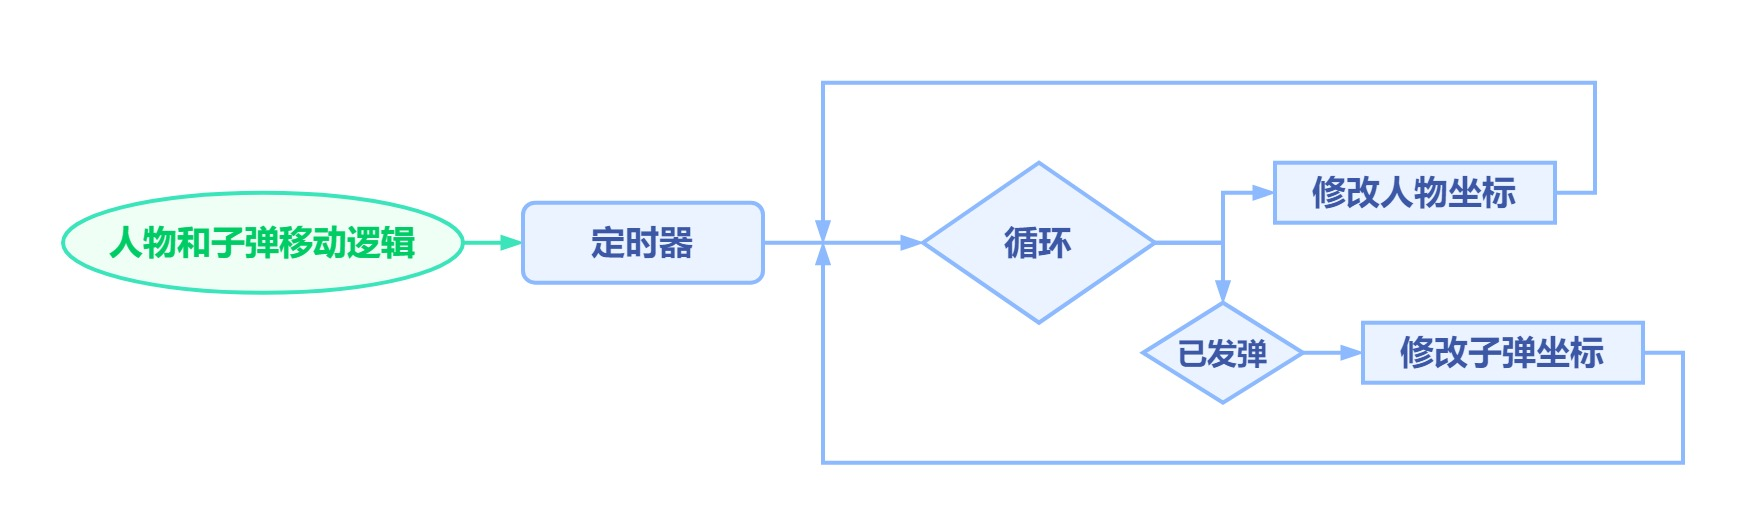
\includegraphics[width=0.8\textwidth]{images/3-5.jpg}
    \caption{人物和子弹移动逻辑示意图}% label 用来在文中索引
\end{figure}
\subsection{道具功能逻辑}
对于两个人物击打道具的判定逻辑都是相同的,只是左边人物的子弹判断的界限是障碍物的左边界,右边人物的子弹判断的界限是障碍物的右边界,所以这里以左边人物为例,介绍击打到不同障碍物时产生的不同效果以及对其的判定逻辑。
\begin{figure}[htbp]
    \vspace{13pt} % 调整图片与上文的垂直距离
    \centering
    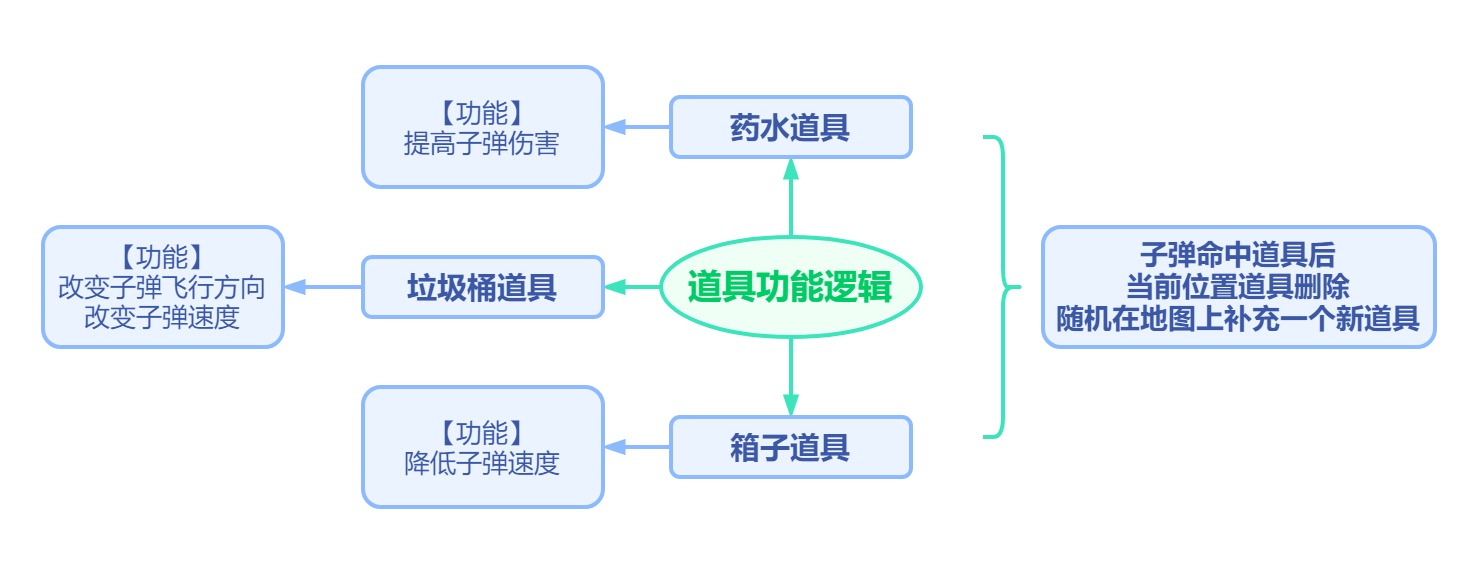
\includegraphics[width=0.8\textwidth]{images/3-6.jpg}
    \caption{道具功能逻辑示意图}% label 用来在文中索引
\end{figure}
\subsubsection{(1)垃圾桶道具}
垃圾桶道具可以实现改变子弹的线路以及速度的功能。对于子弹运行速度的计算,是用x方向的方向标签值乘以x方向的速度,再加上y方向的方向标签值乘以y方向的速度得到的。垃圾桶道具的纵坐标被分为了上中下三个部分,若击打到上半部分,则子弹的y方向标签值设为1,并把此时子弹x方向的速度值直接赋给子弹y方向的速度,从而可以实现子弹以斜向上45度的方向从该道具射出;若击打到中间部分,则子弹的x方向标签值设为-1,即实现了子弹的反弹,子弹有一定概率击打到自己;若击打到下半部分,则子弹的y方向标签值设为-1,并把此时子弹x方向的速度值直接赋给子弹y方向的速度,从而可以实现子弹以斜向下45度的方向从该道具射出。同时垃圾桶道具的功能也支持叠加,从而实现了子弹方向与速度的不断变换。
\begin{lstlisting}[language={[x86masm]Assembler}]
    .if edx>=bound_left && edx<=bound_right	&& ebx<=bound_up &&  ebx>=bound_down;x在范围内						
            .if ebx>=bound_m_up && ebx<=bound_up;上半部 ;speed_y+=speed_x dir_y=1
                mov bullet1.dir_y,1
                mov eax,bullet1.speed_x
                add eax,bullet1.speed_y
                mov bullet1.speed_y,eax
            .endif
            .if ebx>=bound_m_down && ebx<=bound_m_up;中间反弹 dir_x反向
                mov eax,-1
                imul bullet1.dir_x
                mov bullet1.dir_x,eax
            .endif
            .if ebx<=bound_m_down && ebx>=bound_down	;下面反弹
                mov bullet1.dir_y,-1
                mov eax,bullet1.speed_x
                add eax,bullet1.speed_y
                mov bullet1.speed_y,eax
            .endif		
            ;重新更新位置
            invoke getRand,370;150-600为人物x坐标
            add eax,190;范围 190-560
            mov (Prop ptr Prop_Bounce[edi]).pos_x,eax

            invoke getRand,200;160-400为人物上下界
            add eax,180;范围 180-580
            mov (Prop ptr Prop_Bounce[edi]).pos_y,eax
            ;invoke printf,offset coord,eax,eax			
    .endif
\end{lstlisting}
\subsubsection{(2)箱子道具}
箱子道具可以实现子弹的慢速。当子弹射中箱子道具时,子弹x方向的速度值会减4,且该效果可以叠加。为了防止子弹速度减为0,当速度值减小到0以下后,会被设置为速度的最低阈值。
\begin{lstlisting}[language={[x86masm]Assembler}]
    .if edx>=bound_left && edx<=bound_right	&& ebx<=bound_up &&  ebx>=bound_down;x在范围内								
            sub bullet1.speed_x,4
            .if bullet1.speed_x <= 0
                mov bullet1.speed_x,2
            .endif

            ;重新更新位置
            invoke getRand,370;150-600为人物x坐标
            add eax,190;范围 190-560
            mov (Prop ptr Prop_Slow[edi]).pos_x,eax

            invoke getRand,200;160-400为人物上下界
            add eax,180;范围 180-580
            mov (Prop ptr Prop_Slow[edi]).pos_y,eax
            ;invoke printf,offset coord,eax,eax			
    .endif
\end{lstlisting}
\subsubsection{(3)药水道具}
药水道具可以实现子弹的威力增强。普通子弹会对人物造成一滴血的伤害,但若子弹在运行过程中碰到了药水道具,则子弹功能增强,当打到人物时会造成两滴血的伤害,且药水道具的作用可以叠加。如果子弹射中了药水道具,则此时击打到药水道具的标志值就会加1。如果该子弹击中了人物,则人物血量的变化会根据该标志值改变,如果标记值为0,则人物血量减1;如果标记值大于0,则每次人物血量减2,标志值减1,循环直至标记值为0,人物血量判定结束。
\begin{lstlisting}[language={[x86masm]Assembler}]
    .if edx>=bound_left && edx<=bound_right	&& ebx<=bound_up &&  ebx>=bound_down;x在范围内								
            inc	Big_flag1
            ;重新更新位置
            invoke getRand,370;150-600为人物x坐标
            add eax,190;范围 190-560
            mov (Prop ptr Prop_Big[edi]).pos_x,eax

            invoke getRand,200;160-400为人物上下界
            add eax,180;范围 180-580
            mov (Prop ptr Prop_Big[edi]).pos_y,eax
            ;invoke printf,offset coord,eax,eax			
    .endif
\end{lstlisting}
\par
当子弹射击到任意一个道具后,该道具都会消失,然后会再产生随机数,确定更新道具的位置,消失道具与更新道具的类型是相同的。
\subsection{子弹射中判定逻辑}
\begin{figure}[htbp]
    \vspace{13pt} % 调整图片与上文的垂直距离
    \centering
    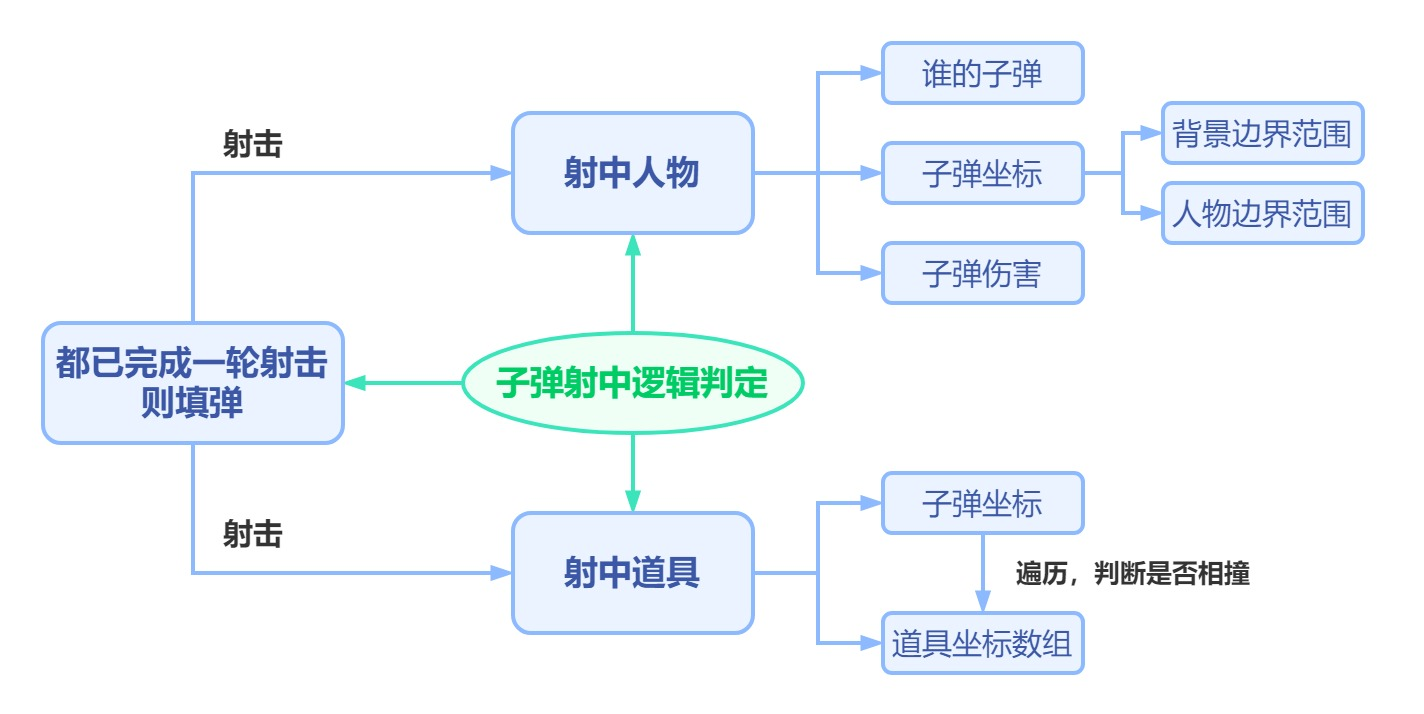
\includegraphics[width=0.7\textwidth]{images/3-7.jpg}
    \caption{子弹射中判定逻辑}% label 用来在文中索引
\end{figure}
\par
\subsubsection{(1)子弹射中人物判定}
根据游戏机制,人物只能由对方的子弹射中。所以我们在设计check\_hit\_person子程序的时候传入了三个参数,分别是子弹的x,y坐标和子弹的归属。对于已发射的子弹而言,我们需要判断子弹的位置是否与人物位置重合,若重合则判定中弹。在中弹的逻辑内我们将person2.is\_hit标志变量设为10,表示人物中弹的状态显示10帧。然后判断子弹是否为加强弹,根据这个更改子弹的伤害值。
\begin{lstlisting}[language={[x86masm]Assembler}]
	.if p==1
	mov eax,person2.pos_y
	sub eax,30
	mov bound_down,eax
	add eax,60
	mov bound_up,eax
	mov eax,person2.pos_x
	sub eax,30
	mov bound_left,eax
	add eax,60
	mov bound_right,eax
	.if ecx<=bound_right && ecx>=bound_left && ebx <= bound_up && ebx >=bound_down
			mov person2.is_hit,10;为了让中弹的样子显示更清楚些,显示10帧
				invoke printf,offset coord,111 ,Big_flag1
				.if  Big_flag1 !=0
					.while Big_flag1>0
						sub person2.life,2
						dec Big_flag1
						invoke printf,offset life2Test,person2.life
					.endw
				.else 
					sub person2.life,1
					invoke printf,offset life2Test,person2.life
				.endif
			.if person2.life == Zero || person2.life == -1 || person2.life == -2 ||person2.life == -3 || person2.life == -4 || person2.life == -5 ||person2.life == -6 ||person2.life == -7 ||person2.life == -8 ||person2.life == -9 ||person2.life == -10
				invoke printf,offset tip,person2.life
				mov person2.life,0
				;invoke game_over
			.endif 
			;填弹逻辑代码在下面展示
            ...
	.endif
	.endif
\end{lstlisting}
\par
对于子弹射出边界,我们根据位置判定若为上下界则反弹,若为左右界则消失。具体的代码实现如下:
\begin{lstlisting}[language={[x86masm]Assembler}]
	.if ecx>= 800 || ecx<=0
		mov bullet1.show,0
		.if person2.bullet == 0 && bullet1.show == 0 && bullet2.show == 0
			mov person1.bullet,1
			mov person2.bullet,1
		.endif
	.endif
	.if (ebx >400 || ebx <160)
			mov eax,-1
			imul bullet1.dir_y
			mov bullet1.dir_y,eax
	.endif
\end{lstlisting}
\par
在射击完子弹后,我们需要判定是否需要填弹,具体的实现逻辑是若玩家1的子弹完成作用时玩家2的子弹夹为0,则两者全部填弹;反之则不做操作。具体的代码实现如下:
\begin{lstlisting}[language={[x86masm]Assembler}]
    mov bullet1.show,0
    .if person2.bullet == 0 && bullet1.show == 0 && bullet2.show == 0
        mov person1.bullet,1
        mov person2.bullet,1
    .endif
\end{lstlisting}
\subsubsection{(2)子弹射中道具判定}
\par
对于子弹射中道具,我们需要获取到子弹的位置,然后去遍历道具数组来判定是否与道具位置相撞。若相撞则根据道具功能来对子弹加以相关特性。这里的判定逻辑不做赘述。遍历道具数组的代码实现如下:
\begin{lstlisting}[language={[x86masm]Assembler}]	
	local bound_up:dword	;up-m_up子弹向上弹
	local bound_m_up:dword	;m_up-m_down 反弹
	local bound_m_down:dword;m_down-down 向下弹
	local bound_down:dword

	local bound_left:dword
	local bound_right:dword
	.if p==1;1发的子弹
		;edx循环计数,ecx,ebx xy坐标
		mov edi,0
		mov ecx,0
		mov ebx,y
		mov edx,x
		;Bounce
		.while ecx<Bounce_Num
			;道具效果已展示,不再赘述
			...
			add edi,type Prop ;Prop大小
			inc ecx	
		.endw
\end{lstlisting}
\subsection{事件响应逻辑}
\begin{figure}[htbp]
    \vspace{13pt} % 调整图片与上文的垂直距离
    \centering
    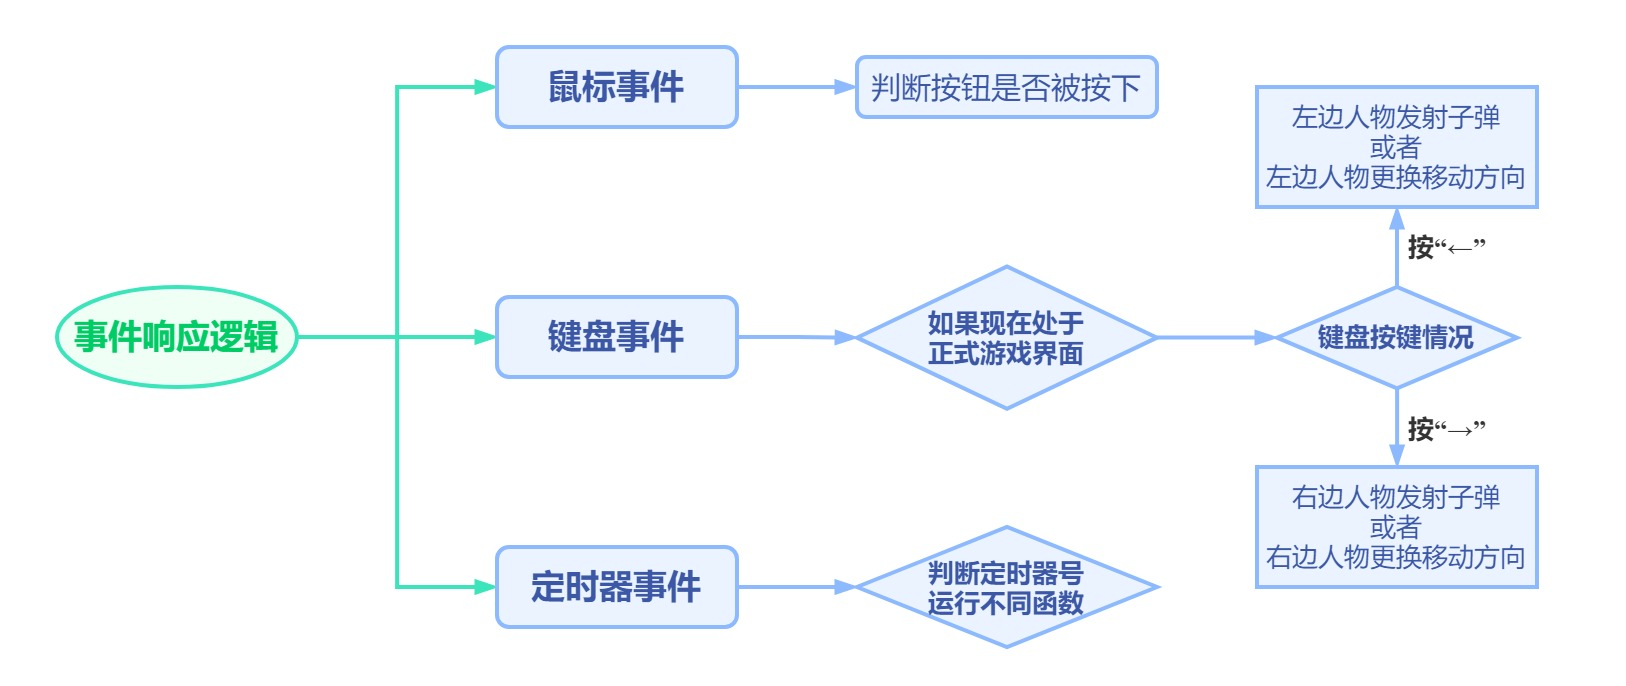
\includegraphics[width=0.8\textwidth]{images/3-8.jpg}
    \caption{事件响应逻辑示意图}% label 用来在文中索引
\end{figure}
\subsubsection{(1)鼠标事件}
单击按钮时,需要判断出当前有鼠标点击,且鼠标点击的位置是否为按钮图片所在的范围。因此使用iface\_mouseEvent和judge\_area子程序来完成按钮的点击效果,实现页面跳转。子程序iface\_mouseEvent是用来判断鼠标是否进行了点击操作的。如果鼠标左键按下,则调用judge\_area子程序对鼠标的点击范围进行判断;在judge\_area子程序中,通过对比start\_button中的范围(即“Start”的范围)和鼠标的坐标大小关系,来确定鼠标坐标是否在“Start”的图片范围之内,如果在的话,就给eax寄存器存值1,否则存0。回归iface\_mouseEvent判断分支,判断eax的值,如果eax为1,说明玩家已经按下“Start”,则通过game\_init子程序完成正式游戏界面的绘制。并且打开定时器0,并以30ms的时间间隔调用计时器0中的函数,实现游戏界面中基本循环的运行。
\begin{lstlisting}[language={[x86masm]Assembler}]
    iface_mouseEvent proc C x:dword,y:dword,button:dword,event:dword
        .if button == LEFT_BUTTON && event == BUTTON_DOWN
            .if	curWindow == 0;当前在主界面
                invoke judge_area,x,y,start_button.left,start_button.right,start_button.top,start_button.bottom
                .if eax==1
                    invoke printf,offset coord,x,y
                    ;游戏开始,设置初始值
                    invoke game_init
                    ;开启循环,30ms触发
                    invoke startTimer,0,30
                .endif
                invoke judge_area,x,y,exit_button.left,exit_button.right,exit_button.top,exit_button.bottom
                .if eax ==1
                    invoke ExitProcess, NULL
                .endif

            .endif
            .if curWindow == 2
                invoke judge_area,x,y,exit_button.left,exit_button.right,exit_button.top,exit_button.bottom
                .if eax ==1
                    invoke ExitProcess, NULL
                .endif
            .endif
        .endif
        ret
    iface_mouseEvent endp
    judge_area proc C uses ebx x:dword,y:dword,left:dword,right:dword,top:dword,bottom:dword
        ;x,y为鼠标按下位置
        mov eax,x
        mov ebx,y
        .if	eax <= left || eax >=right || ebx >= bottom || ebx <= top
            mov eax,0
        .else	
            mov eax,1
        .endif	
        ret
    judge_area endp
\end{lstlisting}
\par
如果在判断鼠标范围时发现鼠标并未在“Start”的范围中点击,则进入“判断是否为‘Exit’按钮”分支。调用judge\_area子程序,通过对比exit\_button中的范围(即”Exit“的范围)和鼠标的坐标大小关系,来确定鼠标是否在“Exit”的范围之内,如果在的话eax此时会变为1,通过判断eax等于1,来决定调用退出进程的子程序。
\subsubsection{(2)键盘事件}
如果当前curWindow为1,即代表是游戏界面,则根据键盘的输入来决定接下来的操作。在该游戏中,键盘总共会有两个输入,即“←”“→”,分别代表左边人物发射子弹和右边人物发射子弹。当判断键盘输入为“←”,且该按键被按下时,首先判断当前人物(即左边人物)是否拥有子弹,如果没有子弹,则更换其运行的方向,不能进行射击行为;如果当前有子弹,则子弹清0,得到当前人物的位置,该位置即为子弹开始显示的坐标,并给子弹设置向右运行的方向标志(即x方向为1,y方向为0),以及子弹每个方向上的速度(即x方向和y方向)。对于子弹运行速度的计算,是用x方向的方向标签值乘以x方向的速度,再加上y方向的方向标签值乘以y方向的速度。最后再把子弹可以显示的标志设为1,确保子弹的正确显示。
\begin{lstlisting}[language={[x86masm]Assembler}]
    iface_keyboardEvent proc C key:dword,event:dword
        .if curWindow == 1
            ;invoke printf,offset coord,person1.dir,person2.dir
            .if key == VK_LEFT && event==BUTTON_DOWN;按下左键,!!注意一定要是按下;不然算两次
                .if person1.bullet==1;有子弹
                    mov person1.bullet,0
                    ;其他子弹操作:设置子弹初始化信息
                    mov eax,person1.pos_x
                    mov bullet1.pos_x,eax
                    mov eax,person1.pos_y
                    mov bullet1.pos_y,eax
                    mov bullet1.dir_x,1
                    mov bullet1.dir_y,0
                    mov bullet1.speed_x,12
                    mov bullet1.speed_y,12
                    mov bullet1.show,1
                .else ;换方向
                    mov eax,-1
                    imul person1.dir
                    mov person1.dir,eax
                .endif
            .endif
            ...
        .endif
        ret
    iface_keyboardEvent endp
\end{lstlisting}
\subsubsection{(3)定时器事件}
注册了定时器事件后,便会根据定时器号选择运行不同的函数。在该游戏中,即当定时器号为0时,则会调用draw\_game的函数,开始游戏界面的绘制。并且根据打开定时器0时对应函数语句的设置,每隔30ms就会调用一次该定时器事件。
\begin{lstlisting}[language={[x86masm]Assembler}]
    iface_timerEvent proc c tid: dword
        .if tid == 0;游戏主循环
            invoke draw/_game
        .endif
        ret
    iface_timerEvent endp
\end{lstlisting}
\section{技术亮点}
在本游戏项目中,我们的程序拥有以下技术亮点:
\begin{itemize}
    \item 使用随机位置算法:我们通过自定义一个seed来在getRand中更新生成的随机数,然后用于位置的坐标中,实现位置的随机化。
    \item 道具的功能多样化,分别具有改变子弹飞行方向、改变子弹速度、改变子弹伤害等效果,这些效果的算法由我们自己编写及实现。
    \item 实现动画效果:通过人眼视觉暂留的原理,对图片的坐标位置和切换逻辑按帧进行规定,使其按帧发生变化,从而人眼获取到的就是动态的动画效果。
    \item 按钮判定:我们没有采用一般的窗口编程的按钮实现和点击事件判定方法,而是通过制作一个按钮的图片,然后判定图片的范围和鼠标单击位置的坐标,如果位置在图片上,则说明点到了此按钮,进入按钮点击后的对应逻辑。
    \item 自定义图片和音乐:本游戏的部分图片素材由我们根据《Among us》游戏的素材自己二次制作而成,另一部分图片素材由我们自己使用Photoshop制作,图片和音乐的风格都符合游戏的风格特色。
\end{itemize}

